For CE development, testing prototypes at room temperature is the first step, as many problems can be identified quickly and without the expense of cryogens.  A quick access test stand with the FEMB connected to an APA inside a shielded environment that is in the same location as the FEMB/ASIC development is invaluable for rapid progress.  Two such facilities are available to DUNE: the shielded room at Fermilab and the 40\% APA test stand at BNL.  In addition, a test dewar design developed by Michigan State University, referred to as the Cryogenic Test System (CTS), allows for additional testing of the FEMBs and ASICs in liquid nitrogen.

The shielded room at Fermilab (see Figure~\ref{fig:shieldedroom}) is 2.5~m tall, and 2~m on each side, with 
a double layer of copper mesh in the walls, floor and ceiling, plus a solid metal plate in the floor all electrically connected to create a faraday cage.  A flexible AC distribution and isolated grounding configuration offers the ability to easily ground the shielded room and refer the associated electronics to either a building ground or a detector ground.  In addition
to evaluating different grounding schemes for the APAs, capacitive coupling issues can be studied by varying the
distance between the floor and a copper plate positioned underneath.   
This room has uniquely easy access to the setup through a shielded door,
and a person can remain inside safely with the door closed and probe the electronics directly while operating
in a shielded environment.  Currently mounted inside are two 35-ton APAs 
with adaptor boards to connect ProtoDUNE electronics.  This installation satisfies the ProtoDUNE grounding and shielding guidelines.  A rough demonstration of the shielding adequacy for our purposes  is the measured noise level of 800~ENC for ProtoDUNE prototype FEMBs.  The same noise level was measured at room temperature in the 40\% APA at BNL for the same FEMBs.

\begin{dunefigure}
[Picture of the shielded room at Fermilab.]
{fig:shieldedroom}
{Picture of the shielded room at Fermilab.}
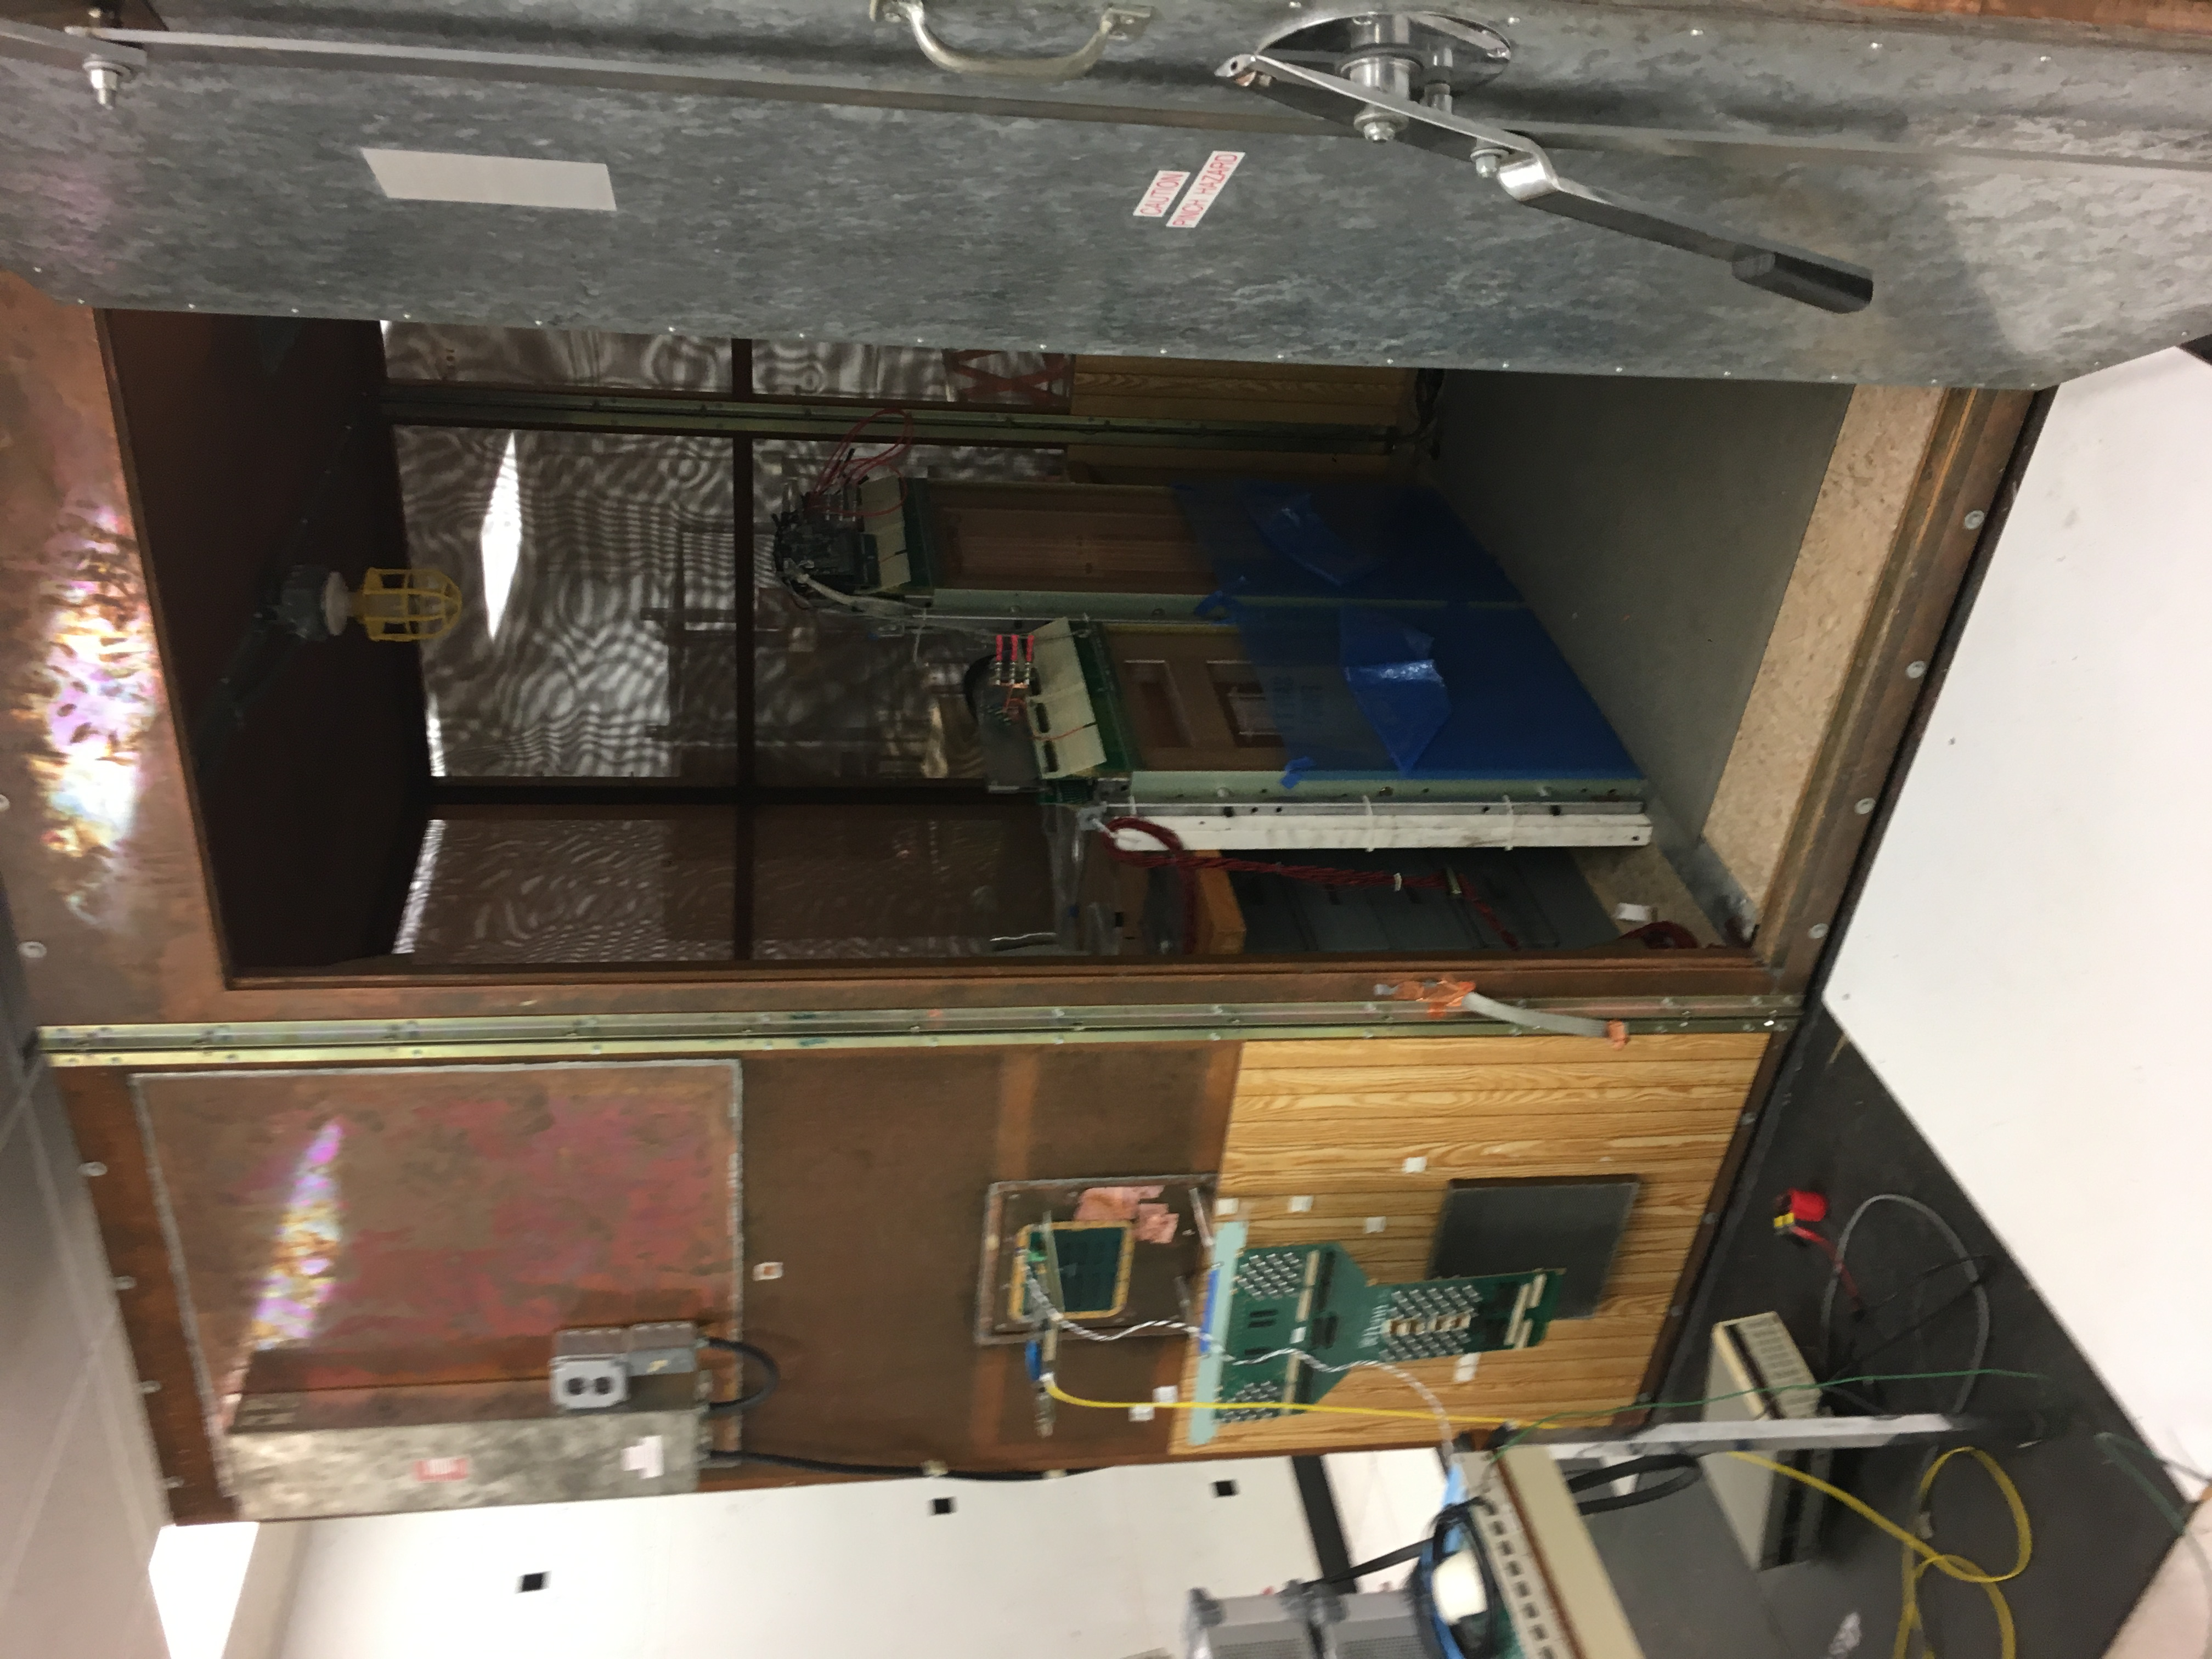
\includegraphics[angle=270,width=0.4\linewidth]{tpcelec-shielded_room.jpg}
\end{dunefigure}

The 40\% APA at BNL is a 2.8~m~$\times$~1.0~m three-plane APA with two layers of 576 wrapped (U/V) wires and one layer of 448 straight (X) wires. It is read out by eight ProtoDUNE-SP FEMBs with the full 7~m ProtoDUNE-SP length data and LV power cables, four on the top and four on the bottom. The readout uses the full CE system for ProtoDUNE-SP, with a prototype CE flange and WIEC, two WIBs and one PTC, as shown in Figure~\ref{fig:tpcelec_40APA}. Detailed integration tests of the CE readout performance while following the DUNE grounding and shielding guidelines have been done at the 40\% APA. Additional input capacitance (equivalent to longer wire length) have been added to a subset of channels to project the ENC performance from the 40\% APA teststand to the ProtoDUNE-SP and SBND detectors. The results from the 40\% APA indicate that, if the new ADC performs as expected, the full CE system as installed on the teststand at BNL will have a noise level in LAr around 500e$^-$ and 600e$^-$ for the collection and induction plane channels, respectively, in line with the CERN cold box tests described in Section~\ref{sec:fdsp-tpc-elec-qa-facilities-coldbox}.

\begin{dunefigure}
[Left: one side of the 40\% APA with 4 FEMBs.  Right: the full CE feedthrough and flange.]
{fig:tpcelec_40APA}
{Left: one side of the 40\% APA with 4 FEMBs.  Right: the full CE feedthrough and flange.}
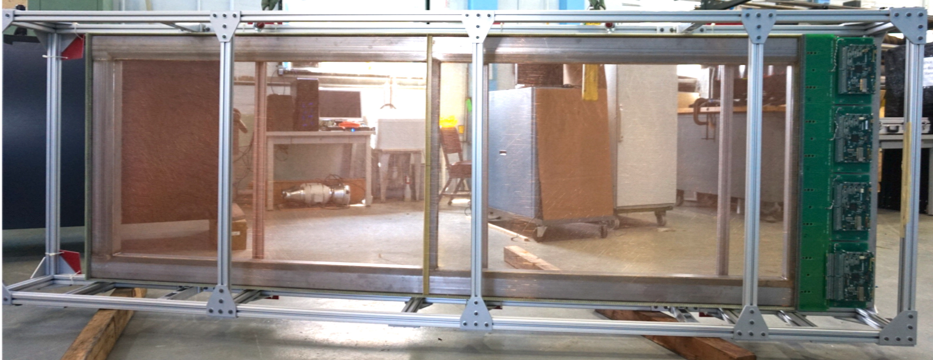
\includegraphics[width=0.72\linewidth]{tpcelec-40-apa.png}
\hspace{3mm}
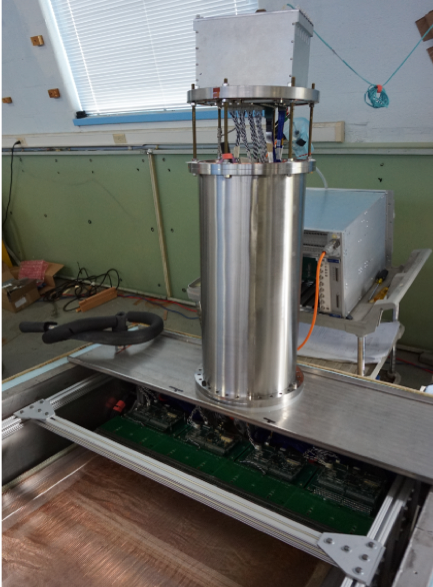
\includegraphics[width=0.2\linewidth]{tpcelec-40-apa-ft.png}
\end{dunefigure}

%\begin{figure}
%    \centering
%    \includegraphics[width=0.9\linewidth]{tpcelec-40-apa-result.png}
%    \caption{ENC (in electrons) as a function of input capacitance (equivalent to input wire length) measured on the 40\% APA. The ENC projections are based on the input wire length of the SBND and ProtoDUNE-SP detectors.}
%    \label{fig:tpcelec_40APA_results}
%\end{figure}

To facilitate testing of individual components and printed circuit boards, members of the Michigan State group have developed the CTS (see Figure~\ref{fig:CTS}).  This system allows a device under test to be cooled down in nitrogen gas, immersed in liquid nitrogen for testing, and then warmed back to room temperature in a nitrogen gas.  This process avoids the condensation of water from air that can otherwise interfere with the tests or damage the test equipment.  A total of nine CTSs will be built and used at consortium member institutions.

\begin{dunefigure}
[Cryogenic Test System: an insulated box is mounted on top of a commercial liquid nitrogen dewar.  Simple controls allow the box to be purged with nitrogen gas and liquid nitrogen to be moved from the dewar to the box and back to the dewar.]
{fig:CTS}
{Cryogenic Test System: an insulated box is mounted on top of a commercial liquid nitrogen dewar.  Simple controls allow the box to be purged with nitrogen gas and liquid nitrogen to be moved from the dewar to the box and back to the dewar.}
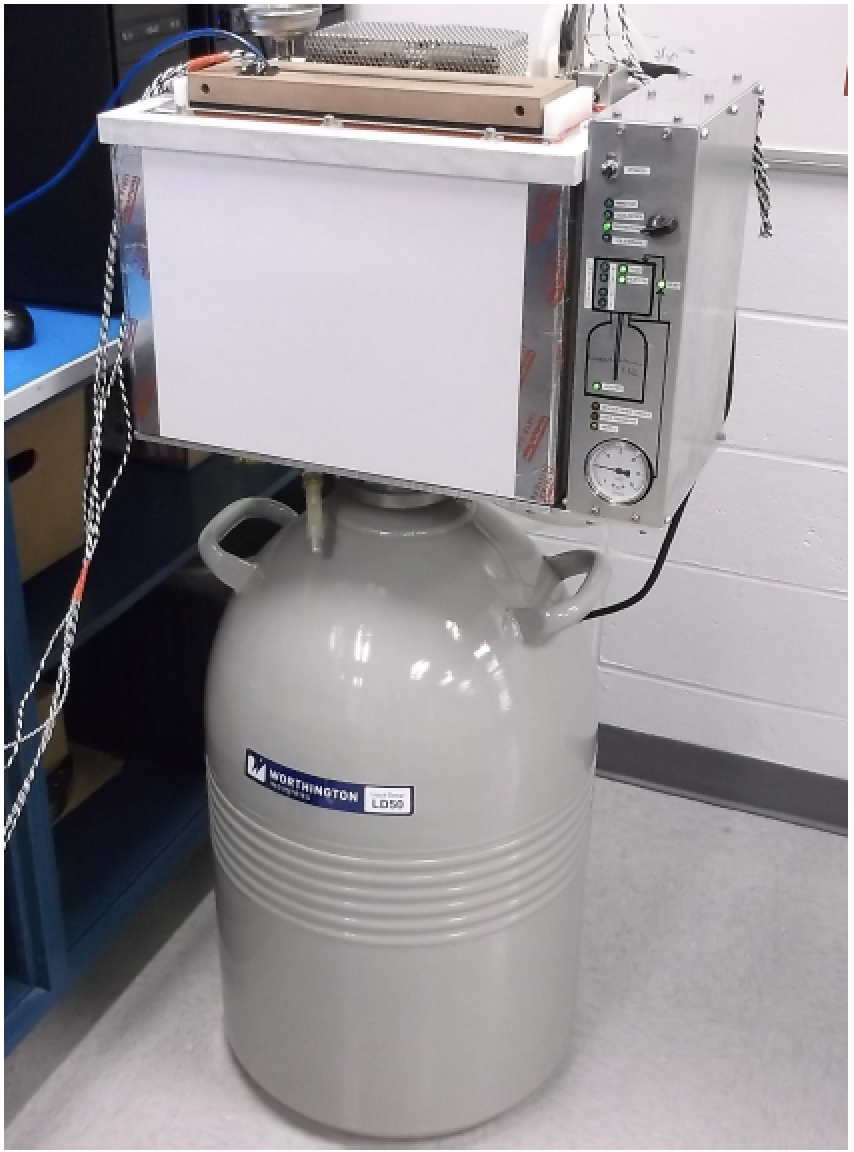
\includegraphics[width=0.4\linewidth]{tpcelec-CTS.png}
\end{dunefigure}
